Obbiettivo: andare a implementare sistema di \textit{visual navigation} per la base robotica in figura ~\ref{fig:BaseRobotica} facendo uso del supporto in figura ~\ref{fig:SupportoRialzato}.

Per il progetto del corso di Robotica è stato implementato un algoritmo in
C++ che, partendo da un’immagine di input, risulta essere in grado di individuare
frecce (sfruttando la libreria OpenCV) composte dalla somma di due differenti forme: un rettangolo, di un certo colore, e un triangolo, di un secondo colore differente
marcatori di un determinato colore di forma circolare , fornendo in output le coordinate dei centri di tali marcatori rispetto ad un sistema di riferimento.
La scelta della forma dei marcatori è ricaduta sulle frecce poichè esse rappresentano \textit{simboli} in grado di fornire una doppia informazione: \textit{direzione e orientamento}, che rappresentano appunto i dati forniti in uscita dalla nostra libreria, la cui struttura a blocchi è rappresentata in figura ~\ref{fig:CodeStructure}.

L’algoritmo è stato sviluppato col presupposto di avere a disposizione un sistema visivo composto da una sola telecamera RGB; inoltre esso fornisce la possibilità di impostare l’angolo che la telecamera forma con l’asse orizzontale e l'altezza della camera stessa rispetto al terreno.


\begin{figure}
	\centering
	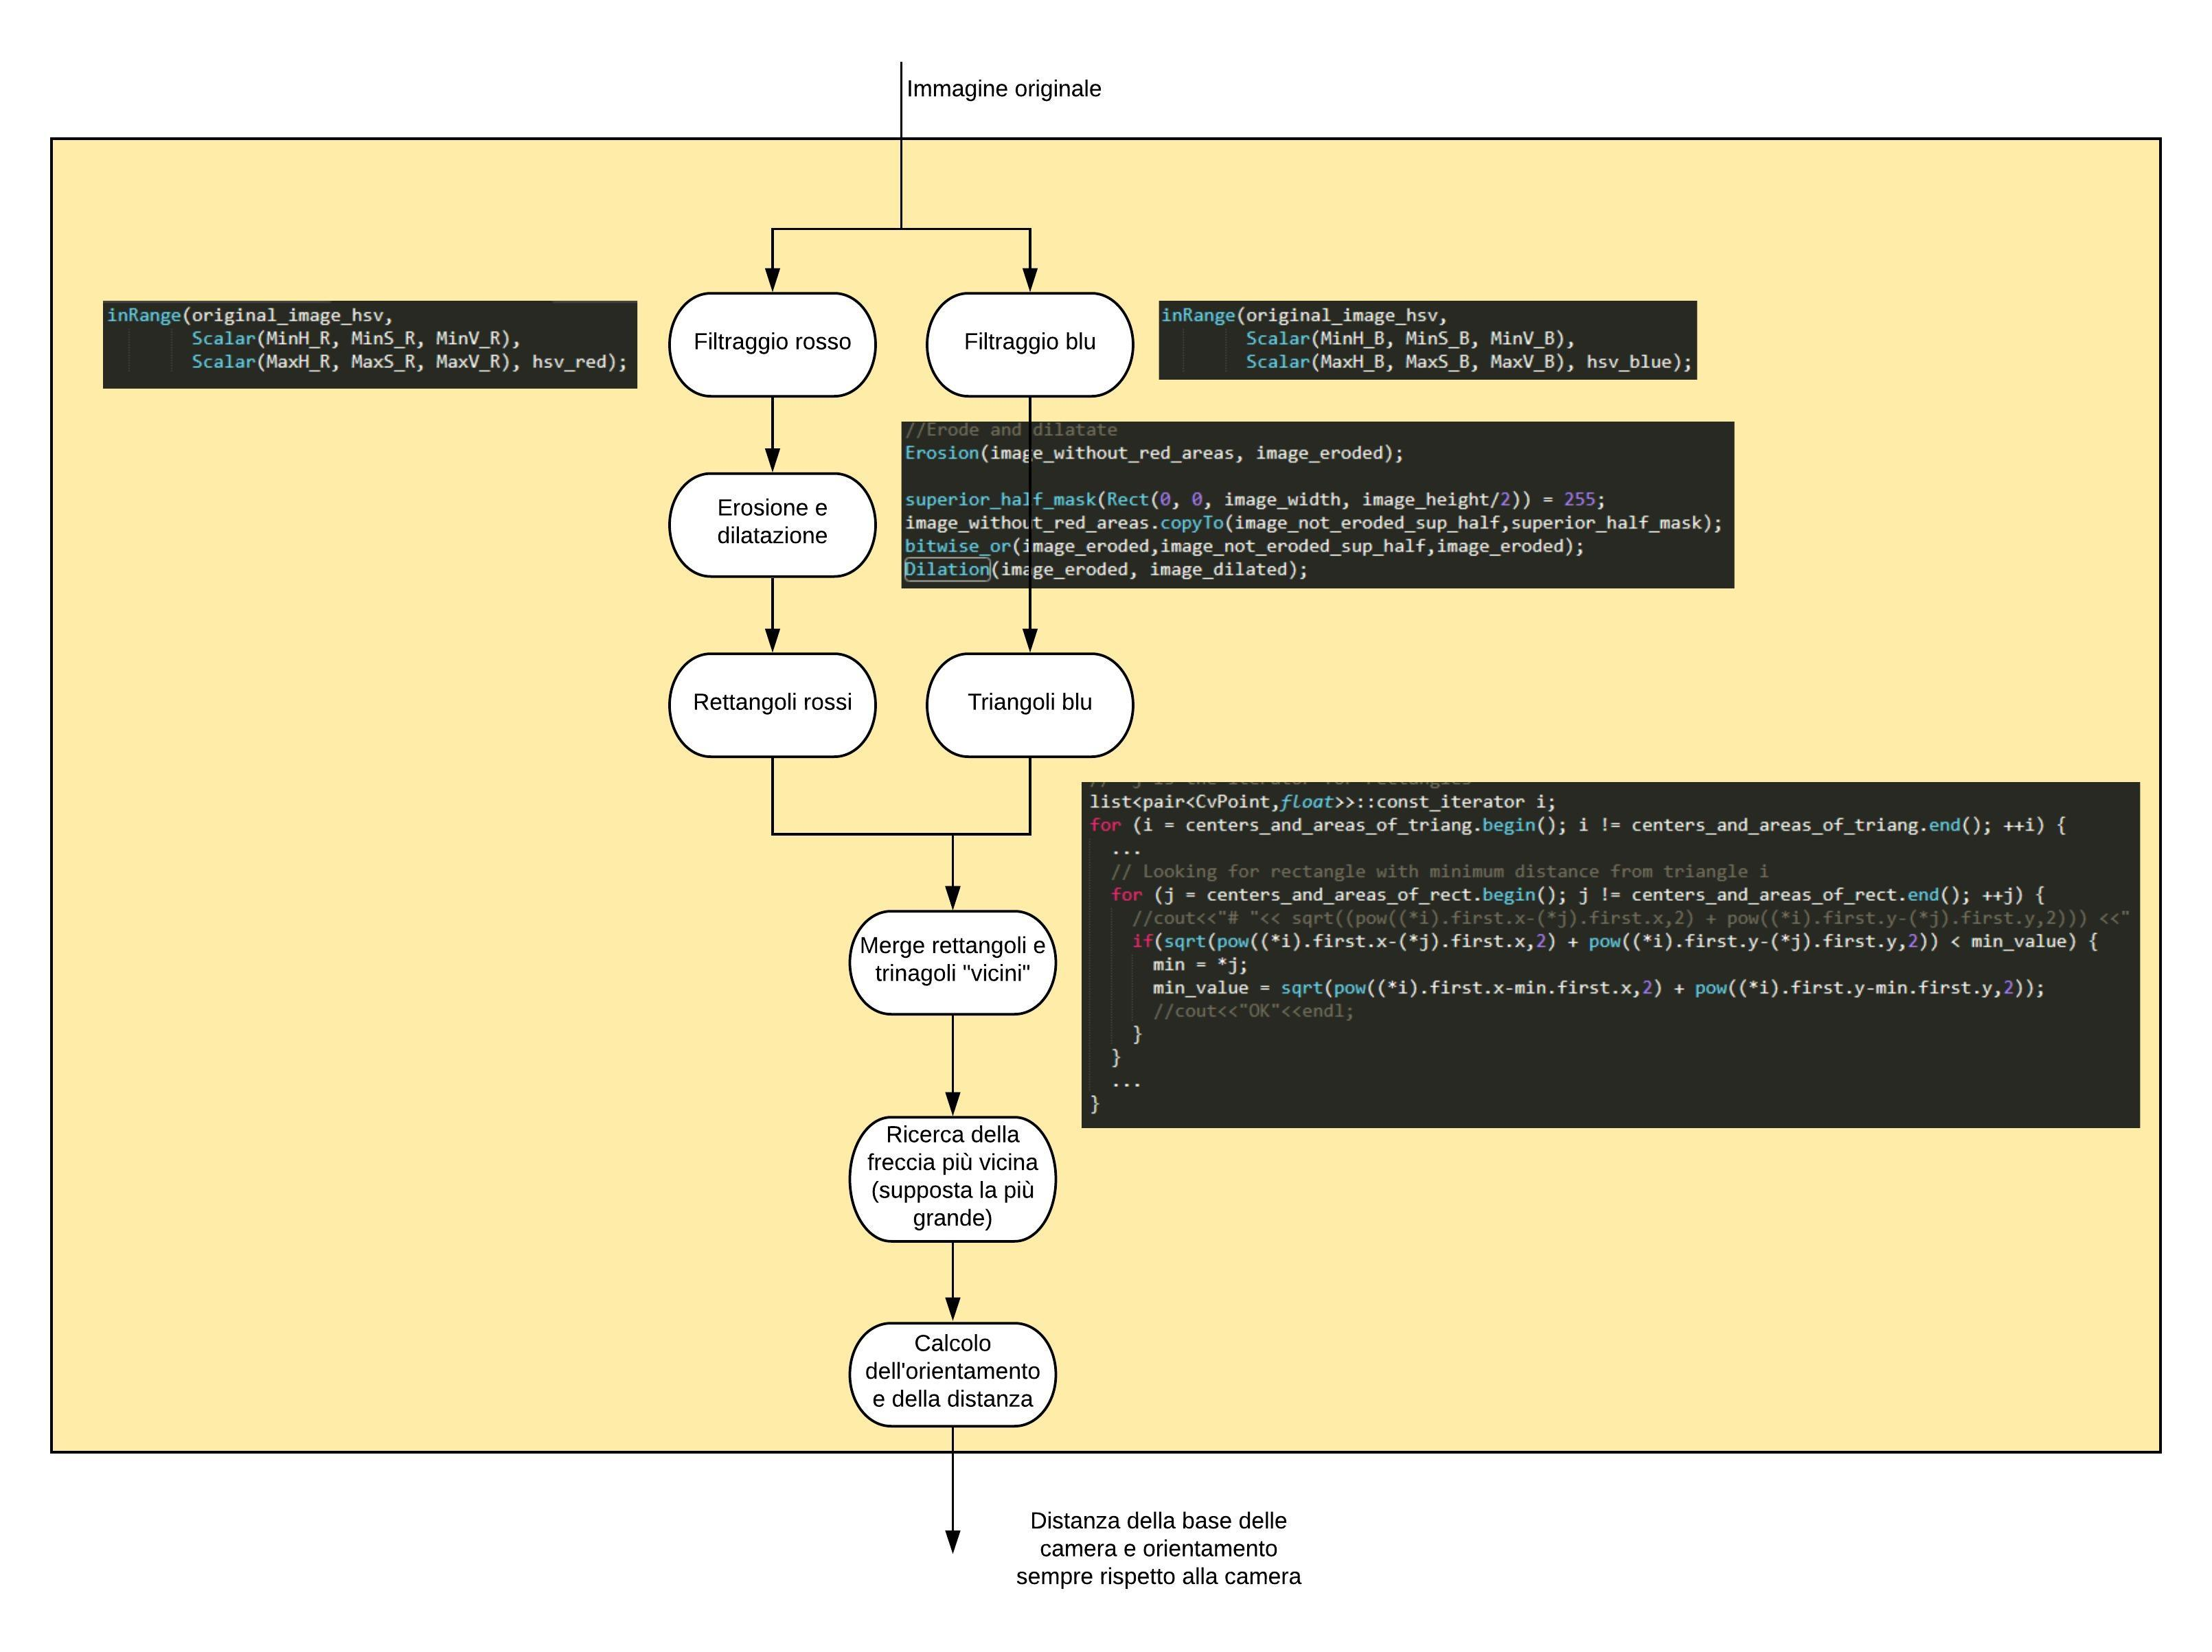
\includegraphics[width=\textwidth]{Immagini/CodeStructure.jpeg}
	\caption{Struttura del codice}
	\label{fig:CodeStructure}
\end{figure}

\begin{figure}
	\centering
	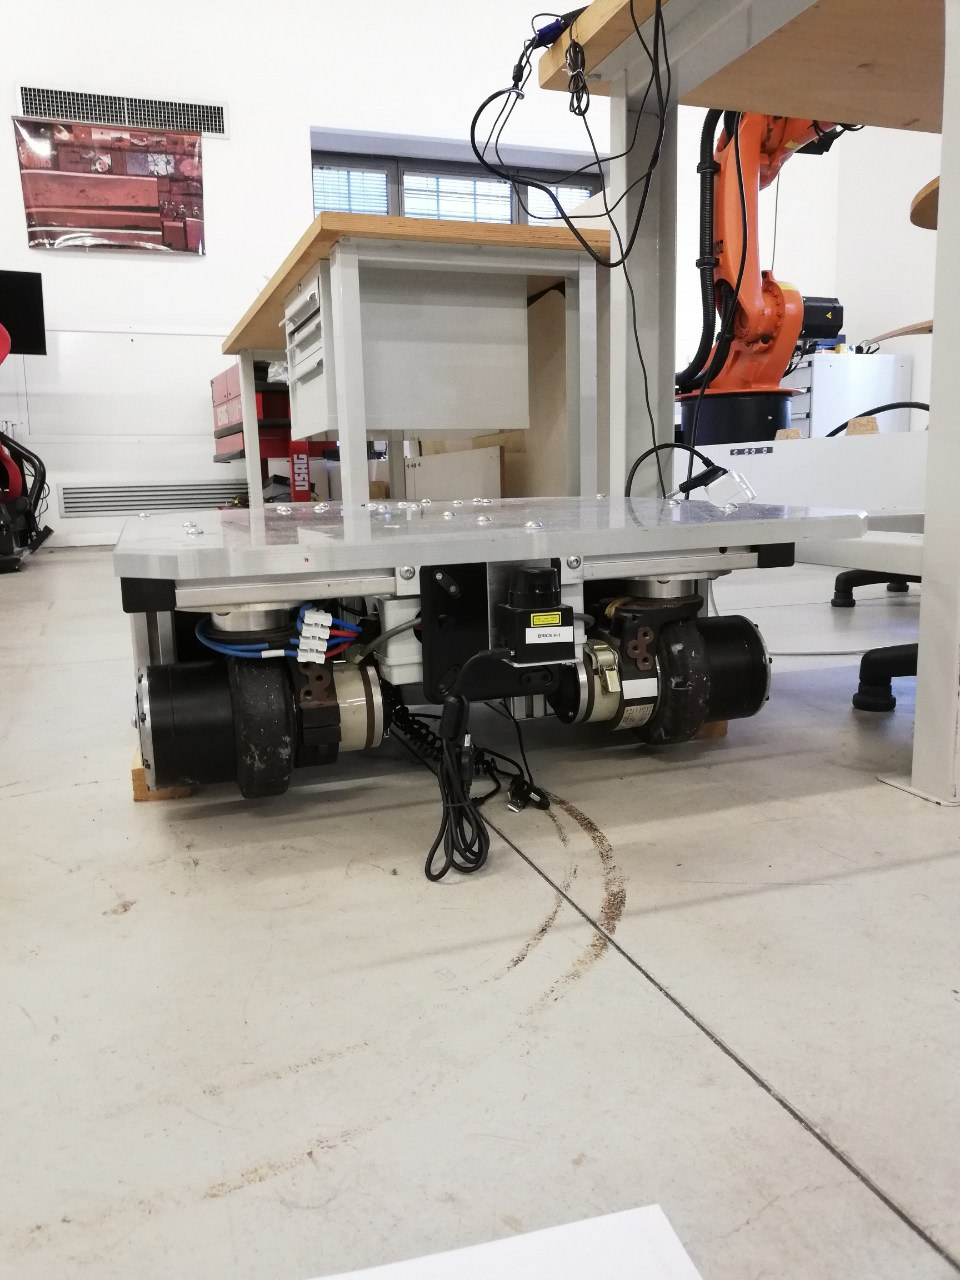
\includegraphics[width=0.5\textwidth]{Immagini/BaseRobotica.jpg}
	\caption{Base robotica addetta alla movimentazione}
	\label{fig:BaseRobotica}
\end{figure}

\begin{figure}
	\centering
	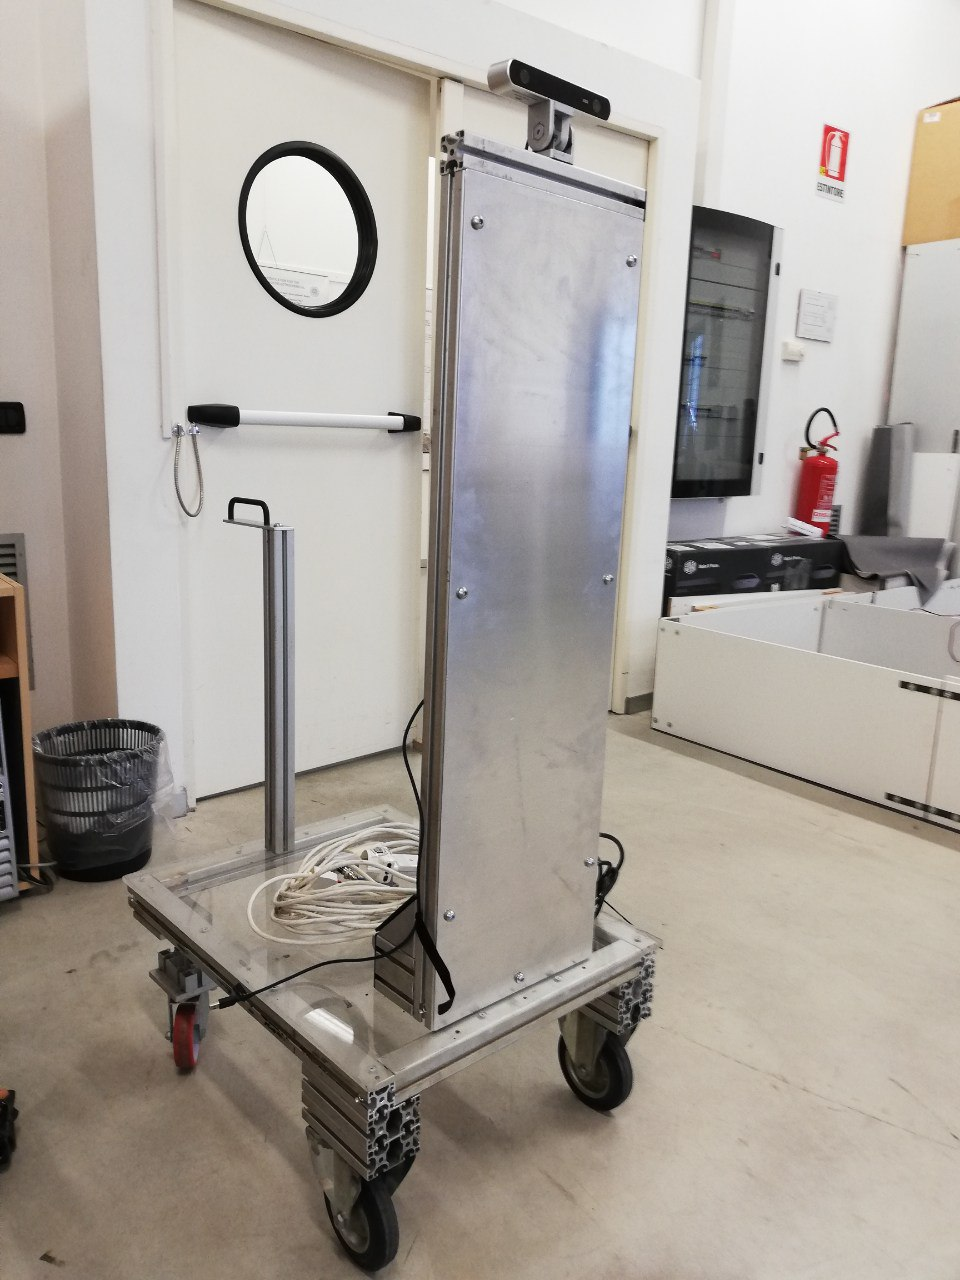
\includegraphics[width=0.5\textwidth]{Immagini/SupportoCamera.jpg}
	\caption{Base verticale sulla quale andare ad inserire la camera}
	\label{fig:SupportoRialzato}
\end{figure}